\documentclass[11pt]{beamer}


\beamertemplatenavigationsymbolsempty

\usetheme{Madrid}

% Colours
\newcommand{\primaryBlue}{blue}
\newcommand{\primaryRed}{red}
\newcommand{\primaryGreen}{green!60!black}
\newcommand{\primaryYellow}{yellow}


\newcommand{\colorVertex}{\primaryBlue!50!white}
\newcommand{\colorEdge}{black}
\newcommand{\colorFace}{\primaryYellow}
\newcommand{\colorDarkFace}{\primaryYellow!80!black}
\newcommand{\colorEdgeBack}{magenta!20!white}

\newcommand{\colorVertexNode}{\colorVertex}

\newcommand{\colorEdgeA}{\primaryBlue}
\newcommand{\colorEdgeB}{\primaryRed}
\newcommand{\colorEdgeC}{\primaryGreen}


\newcommand{\colorFaceA}{cyan}
\newcommand{\colorFaceB}{magenta}
\newcommand{\colorFaceC}{orange}

\newcommand{\colorRed}{\primaryRed}


\newcommand{\graphColorA}{purple}
\newcommand{\graphColorB}{\primaryGreen}
\newcommand{\graphColorC}{orange}
\newcommand{\graphColorD}{black}
\newcommand{\graphColorE}{\primaryBlue}

\newcommand{\colorGraphA}{\graphColorA}
\newcommand{\colorGraphB}{\graphColorB}
\newcommand{\colorGraphC}{\graphColorE}

\newcommand{\colorGraphAlpha}{\graphColorB}
\newcommand{\colorGraphBeta}{\graphColorE}
\newcommand{\colorGraphGamma}{\graphColorC}
\newcommand{\colorGraphDelta}{\graphColorD}

% Graphic support

\usepackage{amsmath, amssymb, amsfonts} % Standard Math-stuff

\usepackage{tikz}
\usetikzlibrary{calc}
\usetikzlibrary{positioning}
\usetikzlibrary{arrows, decorations.pathreplacing, calc, decorations.pathmorphing, shapes}


% Now we define the global styles

% We start by defining the default colours of vertices, edges and faces
\newcommand{\vertexColor}{\colorVertex}
\newcommand{\edgeColor}{\colorEdge}
\newcommand{\faceColor}{\colorFace}
% If we want to shade a surface with two colours, we need an alternative
\newcommand{\faceColorDark}{\colorDarkFace}

\newcommand{\vSize}{2pt}    % How big are the vertex circles (if drawn)?


\tikzset{vertex/.style = {\vertexColor}}
\tikzset{edge/.style = {\edgeColor, thick}}
\tikzset{edgeBackground/.style = {fill=\colorEdgeBack}}
\tikzset{face/.style = {fill=\faceColor, draw=\edgeColor}}
% The face style for the alternative colouring. The colour changes if
% \differentColors is defined.
\tikzset{faceDark/.style = {fill=\faceColorDark, draw=\edgeColor}}


% Custom command to draw an edge between two points
% First two parameters are the names of the points (no brackets)
% Third parameter is the name of the edge
\newcommand{\drawEdge}[3]{
    \node[edgeBackground] at ($1/2*(#1)+1/2*(#2)$) {#3};
}

% Custom command to draw a bi-arrow with a sharp bend
% Optional: If you want to have a bi-arrow between planes, this is the (Back)-point
% First parameter: Draw options
% Second parameter: Start point
% Third parameter: Middle point
% Fourth parameter: Final point
\newcommand<>{\planEdge}[5][(0,0)]{
    \uncover#6{
        \draw[#2,<-] ($0.5*#1+#3$) -- ($0.5*#1+#4$);
        \draw[#2,->] ($0.5*#1+#4$) -- ($0.5*#1+#5$);
    }
}

\newcommand{\planeOp}{0.8}

% Draw a plane behind the second and third parameters (defined by first one)
% Optinal argument: colour
\newcommand<>{\behindPlane}[4][black]{
    \uncover#5{
        \filldraw[fill=#1!20!white,draw=#1!50!white,opacity=\planeOp] 
            (#3) -- (#4) -- ($(#4)+(#2)$) -- ($(#3)+(#2)$) -- cycle;
        \draw[#1] (#3) -- (#4);
    }
}

% 1: colour (default black)
% 2: movement backwards
% 3: first vertex
% 4: second vertex
% 5: bend angle
\newcommand<>{\curvedPlane}[5][black]{
    \uncover#6{
        \filldraw[fill=#1!20!white,draw=#1!50!white,opacity=\planeOp]
            (#3) to[bend left=#5] (#4) -- ($(#4)+(#2)$) to[bend right=#5] ($(#3)+(#2)$) -- cycle;
        \draw[#1] (#3) to[bend left=#5] (#4);
    }
}
    
\tikzset{graphVertex/.style={circle,fill=gray!70!white,inner sep=1.5pt}}

% Sometimes we want to implement different behaviour for the generated 
% HTML-pictures (for example, shading is not supported in HTML).
% For that we define a macro to check whether we run the code with
% htlatex. The code comes from 
% https://tex.stackexchange.com/questions/93852/what-is-the-correct-way-to-check-for-latex-pdflatex-and-html-in-the-same-latex
\makeatletter
\edef\texforht{TT\noexpand\fi
  \@ifpackageloaded{tex4ht}
    {\noexpand\iftrue}
    {\noexpand\iffalse}}
\makeatother


\usepackage{hyperref}


\author[M. Baumeister]{Markus Baumeister\\ \vspace{1mm} \small{(j/w Alice Niemeyer)}}
\title{Simplicial surfaces in GAP}
\institute[RWTH Aachen]{Lehrstuhl B für Mathematik\\RWTH Aachen University}
\date{30.08.2017}

\begin{document}
\begin{frame}[fragile]{Folding graph}
    \begin{itemize}
        \item<2->Vertices are folding complexes (modelling folding states)
        \item<3->Edges are folding plans connecting two folding complexes
    \end{itemize}

    \begin{center}
        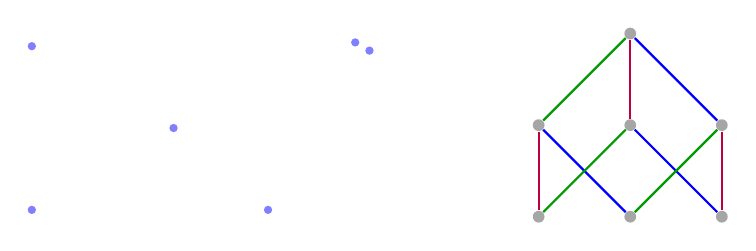
\begin{tikzpicture}[graphEdge/.style={thick}]
            \def\len{1.2}
            \def\off{10}
            \def\dist{0.5}

            \coordinate (Z) at (0,0);
            \coordinate (Back) at (0.4*\len,0.2*\len);
            \foreach \i in {0,1,2}
                \coordinate (P\i) at (120*\i:\len);


            \def\fgA{\colorGraphB}
            \def\fgB{\colorGraphA}
            \def\fgC{\colorGraphC}

            \planEdge<5->[(Back)]{graphEdge,\fgB}{(120+\off:0.5*\len)}{(180:\dist*\len)}{(240-\off:0.5*\len)}
            \behindPlane<4->{Back}{Z}{P2}
            \behindPlane<4->{Back}{Z}{P1}
            \planEdge<5->[(Back)]{graphEdge,\fgC}{(-120+\off:0.5*\len)}{(-60:\dist*\len)}{(-\off:0.5*\len)}
            \behindPlane<4->{Back}{Z}{P0}
            \planEdge<5->[(Back)]{graphEdge,\fgA}{(\off:0.5*\len)}{(60:\dist*\len)}{(120-\off:0.5*\len)}

            \uncover<4->{
                \foreach \i in {2,1,0}{
                    \fill[\vertexColor] (P\i) circle (1.5pt);
                }
            }

            \begin{scope}[xshift=3cm]
                \coordinate (Z) at (0,0);
                \coordinate (Back) at (0.4*\len,0.2*\len);
                \coordinate (P0) at (60-0.5*\off:\len);
                \coordinate (P1) at (60+0.5*\off:\len);
                \coordinate (P2) at (240:\len);

                \uncover<6->{
                    \planEdge[(Back)]{graphEdge,\fgB}{(240-\off:0.5*\len)}{(150:0.4*\len)}{(60+2*\off:0.5*\len)}
                    \behindPlane{Back}{Z}{P1}
                    \behindPlane{Back}{Z}{P2}
                    \behindPlane{Back}{Z}{P0}
                    \planEdge[(Back)]{graphEdge,\fgC}{(240+\off:0.5*\len)}{(-30:0.4*\len)}{(60-2*\off:0.5*\len)}

                    \foreach \i in {0,1,2}
                        \fill[\vertexColor] (P\i) circle (1.5pt);
                }
            \end{scope}

            % Second part
            \begin{scope}[xshift=7cm]
                \uncover<6->{
                    \coordinate[graphVertex] (Top) at (0,\len);
                    \node[graphVertex] (Mid) [below=of Top] {};
                    \node[graphVertex] (MidLeft) [left=of Mid] {};
                    \node[graphVertex] (MidRight) [right=of Mid] {};
                }
                \uncover<7->{
                    \node[graphVertex] (DownLeft) [below=of MidLeft] {};
                    \node[graphVertex] (Down) [below=of Mid] {};
                }
                \uncover<8->{
                    \node[graphVertex] (DownRight) [below=of MidRight] {};
                }

                \uncover<6->{
                    \draw[graphEdge, \fgA] (Top) -- (MidLeft);
                    \draw[graphEdge, \fgB] (Top) -- (Mid);
                    \draw[graphEdge, \fgC] (Top) -- (MidRight);
                }
                \uncover<7->{
                    \draw[graphEdge, \fgB] (MidLeft) -- (DownLeft);
                    \draw[graphEdge, \fgC] (MidLeft) -- (Down);
                }
                \uncover<8->{
                    \draw[graphEdge, \fgA] (Mid) -- (DownLeft);
                    \draw[graphEdge, \fgC] (Mid) -- (DownRight);
                    \draw[graphEdge, \fgA] (MidRight) -- (Down);
                    \draw[graphEdge, \fgB] (MidRight) -- (DownRight);
                }
            \end{scope}
        \end{tikzpicture}
    \end{center}

    % Second diagram
    \begin{center}
        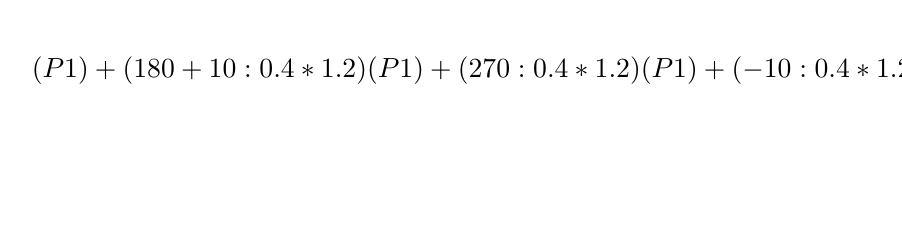
\begin{tikzpicture}[graphEdge/.style={thick}]
            \def\fgA{\colorGraphAlpha}
            \def\fgB{\colorGraphBeta}
            \def\fgC{\colorGraphGamma}
            \def\fgD{\colorGraphDelta}

            % First picture
            \def\len{1.2}
            \def\off{10}
            \def\scal{0.4}

            \foreach \i in {0,1,2,3}
                \coordinate (P\i) at (\i*\len,0);

            \coordinate (Back) at (0.4*\len,0.2*\len);

            \planEdge<10->[(Back)]{graphEdge,\fgB}{($(P1)+(180+\off:\scal*\len)$)}{($(P1)+(270:\scal*\len)$)}{($(P1)+(-\off:\scal*\len)$)}
            \planEdge<10->[(Back)]{graphEdge,\fgD}{($(P2)+(180+\off:\scal*\len)$)}{($(P2)+(270:\scal*\len)$)}{($(P2)+(-\off:\scal*\len)$)}
            \behindPlane<9->{Back}{P0}{P1}
            \behindPlane<9->{Back}{P1}{P2}
            \behindPlane<9->{Back}{P2}{P3}
            \planEdge<10->[(Back)]{graphEdge,\fgA}{($(P1)+(180-\off:\scal*\len)$)}{($(P1)+(90:\scal*\len)$)}{($(P1)+(\off:\scal*\len)$)}
            \planEdge<10->[(Back)]{graphEdge,\fgC}{($(P2)+(180-\off:\scal*\len)$)}{($(P2)+(90:\scal*\len)$)}{($(P2)+(\off:\scal*\len)$)}


            \uncover<9->{
                \foreach \i in {0,1,2,3}
                    \fill[\vertexColor] (P\i) circle (1.5pt);
            }

            \begin{scope}[yshift=-1.3cm]
                \def\above{0.1}

                \coordinate (P1) at (\len,0);
                \coordinate (P1Alt) at ($(P1)+(0,0.5*\above)$);
                \coordinate (P2) at (2*\len,0);
                \coordinate (P3) at (3*\len,0);
                \coordinate (P0) at (1.8*\len,\above);

                \coordinate (Back) at (0.4*\len,0.2*\len);
                
                \planEdge<11->[(Back)]{graphEdge,\fgD}
                    {($(P2)+(180+\off:\scal*\len)$)}
                    {($(P2)+(270:\scal*\len)$)}
                    {($(P2)+(-\off:\scal*\len)$)}
                \behindPlane<11->{Back}{P1}{P2}
                \behindPlane<11->{Back}{P2}{P3}
                \behindPlane<11->{Back}{P1}{$(P1)+(0,\above)$}
                \behindPlane<11->{Back}{$(P1)+(0,\above)$}{P0}
                \planEdge<11->[(Back)]{graphEdge,\fgC,dashed}
                    {($(P2)+(180-\off:\scal*\len)$)}
                    {($(P2)+(90:\scal*\len)$)}
                    {($(P2)+(\off:\scal*\len)$)}
                
                \uncover<11->{
                    \foreach \p in {P1Alt,P0,P2,P3}
                        \fill[\vertexColor] (\p) circle (1.5pt);
                }
            \end{scope}


            \begin{scope}[xshift=6cm, yshift=-0.4cm]
                \uncover<13->{
                    \coordinate[graphVertex] (B1) at (-\len,-\len);
                }
                \foreach \i/\j/\pos in {1/2/12,2/3/14,3/4/14,4/5/12,5/6/14}{
                    \uncover<\pos->{
                        \node[graphVertex] (B\j) [right=of B\i] {};
                    }
                    \coordinate (H\i\j) at ($(B\i)!0.5!(B\j)$);
                }

                \uncover<11->{
                    \foreach \i/\j in {1/2,2/3,4/5,5/6}{
                        \node[graphVertex] (M\i\j) [above=of H\i\j] {};
                    }

                    \coordinate (M34) at ($(M23)!0.5!(M45)$);
                    \node[graphVertex] (Top) [above=of M34] {};
                }

                \uncover<11->{
                    \draw[graphEdge, \fgA] (Top) -- (M12);
                    \draw[graphEdge, \fgB] (Top) -- (M45);
                    \draw[graphEdge, \fgC] (Top) -- (M56);
                    \draw[graphEdge, \fgD] (Top) -- (M23);
                }

                \uncover<12->{
                    \draw[graphEdge, \fgD] (B2) -- (M12);
                    \draw[graphEdge, \fgA] (B2) -- (M23);
                    \draw[graphEdge, \fgB] (B5) -- (M56);
                    \draw[graphEdge, \fgC] (B5) -- (M45);
                }

                \uncover<13->{
                    \draw[graphEdge, \fgC,dashed] (B1) -- (M12);
                }

                \uncover<14->{
                    \draw[graphEdge, \fgB,dashed] (B3) -- (M23);
                    \draw[graphEdge, \fgD,dashed] (B4) -- (M45);
                    \draw[graphEdge, \fgA,dashed] (B6) -- (M56);
                }
            \end{scope}
        \end{tikzpicture}
    \end{center}
\end{frame}


\end{document}
